%======================================================================
\section{Hardware e placa de circuito impresso}\label{sec:pcb}
%======================================================================
\subsection{Plataforma: ESP32-S3-DevKitC-1}

As duas placas usam a ESP32-S3-DevKitC-1~\cite{esp32s3}. O ESP32-S3 tem dois núcleos
Xtensa LX7 de até 240\,MHz, 512\,KB de SRAM, Wi-Fi de 2,4\,GHz e Bluetooth LE, dois ADCs de
12 bits, o controlador CAN do próprio chip (TWAI), o periférico RMT que acende o LED
WS2812 e um coprocessador de ultrabaixo consumo (ULP RISC-V). A DevKit traz o módulo com a
antena, o regulador de 3,3\,V, uma ponte USB--serial e a USB nativa do chip. Os dois núcleos
pesaram na escolha: o rádio e os protocolos ficam num núcleo e o tempo real (amostragem,
sensores) no outro (Seção~\ref{sec:tasks}).

\subsection{Uma PCB para as duas placas}

O hub e a pulseira usam \textbf{uma só PCB}: uma placa-base em que a DevKit é encaixada e
que leva os periféricos dos dois. Só o firmware muda: o hub usa as portas, o PIR e o LM35; a
pulseira usa o MPU-6050 e o botão; os dois podem usar o CAN e o LED da DevKit
(Figura~\ref{fig:pcb_blocos}).

A placa é única por duas razões. A disciplina imprime um único modelo de placa por grupo, então
as duas placas do sistema tinham de caber num mesmo projeto. E, por ser um protótipo, juntar o
hub e a pulseira numa placa só não atrapalha os testes: as duas funções usam a mesma DevKit,
nenhuma divide pino com a outra, e o firmware escolhe o que cada uma liga.

\begin{figure}[H]
\centering
\resizebox{\linewidth}{!}{% Blocos da PCB única: o que cada placa usa em volta da DevKit.
\begin{tikzpicture}[font=\scriptsize]
  \node[draw=black!70, fill=black!5, thick, rounded corners=2pt, minimum width=3.0cm, minimum height=6.6cm,
        align=center, font=\footnotesize] (dk) at (0,0) {\textbf{ESP32-S3}\\\textbf{DevKitC-1}\\(U1, encaixada)\\[4pt]LED WS2812\\(GPIO 38/48)};

  % lado esquerdo (J1 da DevKit): analógico e entradas do quarto, CAN, alimentação
  \tikzset{esq/.style={bloco=#1, text width=4.3cm, align=left, anchor=east}, dir/.style={bloco=#1, text width=4.1cm, align=left, anchor=west}}
  \node[esq=corhub] (an) at (-2.6,2.4) {\textbf{GPIO 4}: LM35DZ $\to$ LM358 (G = 5,55) $\to$ filtro RC (U2, U3, R1--R3, C3)};
  \node[esq=corhub] (pir) at (-2.6,1.0) {\textbf{GPIO 8}: PIR HC-SR501 (J2), com R4 em série};
  \node[esq=corhub] (portas) at (-2.6,-0.2) {\textbf{GPIO 11, 12}: portas 1 e 2, reed MC-38 (J3, J4)};
  \node[esq=corambas] (can) at (-2.6,-1.6) {\textbf{GPIO 13, 14}: transceptor CAN SN65HVD230 (J1) e barramento CANH, CANL, GND (J7)};
  \node[esq=cinza] (pwr) at (-2.6,-3.0) {\textbf{5V}: USB-C (J6) $\to$ C8 $\to$ D1 1N5819};
  % lado direito (J3 da DevKit): I2C, botão, pontos de teste
  \node[dir=corvest] (mpu) at (2.6,2.0) {\textbf{GPIO 1, 2 (I²C) e 17 (INT)}: MPU-6050 (J5); par do ULP, INT em RTC GPIO};
  \node[dir=corvest] (bt) at (2.6,0.5) {\textbf{GPIO 18}: botão ``estou bem'' (SW1)};
  \node[dir=cinza] (tp) at (2.6,-1.0) {pontos de teste: 5V, 3V3, GND, saída do LM358, CANH, CANL};
  \node[dir=cinza] (livre) at (2.6,-2.5) {livres: 6, 7 (analógico), 9, 10 (portas 3 e 4), 21 e 39--42 (expansão)};

  \foreach \n in {an,pir,portas,can,pwr} {\draw[thick, black!60] (\n.east) -- (\n.east -| dk.west);}
  \foreach \n in {mpu,bt,tp,livre} {\draw[thick, black!60] (\n.west) -- (\n.west -| dk.east);}

  % legenda
  \node[anchor=north, align=left, font=\scriptsize] at (0,-3.7) {%
    \tikz\fill[corhub!40] (0,0) rectangle (0.3,0.2); só o hub \quad
    \tikz\fill[corvest!40] (0,0) rectangle (0.3,0.2); só a pulseira \quad
    \tikz\fill[corambas!40] (0,0) rectangle (0.3,0.2); os dois (na pulseira, só em bancada) \quad
    \tikz\fill[cinza!40] (0,0) rectangle (0.3,0.2); comum};
\end{tikzpicture}
}
\caption{Blocos da PCB v1 em volta da DevKit, com o GPIO de cada um.}
\label{fig:pcb_blocos}
\end{figure}

\subsection{Mapa de pinos}\label{sec:pinos}

Como as duas placas compartilham a PCB, nenhuma função divide pino com outra. A escolha
seguiu regras tiradas da documentação do ESP-IDF para o ESP32-S3 e da aula de projeto de
PCB (Tabela~\ref{tab:regras_pinos}): não usar um pino que uma função do chip ligada no futuro
tomaria, mesmo que hoje não haja conflito.

\begin{table}[H]
\centering
\caption{Regras de escolha dos pinos.}
\label{tab:regras_pinos}
\small
\begin{tabular}{@{}l>{\raggedright\arraybackslash}p{2.0cm}>{\raggedright\arraybackslash}p{10.2cm}@{}}
\toprule
Nível & GPIO & Por quê \\
\midrule
nunca & 0, 3, 45, 46 & pinos de \textit{strapping}: o nível no boot muda o modo da placa \\
nunca & 19, 20 & USB nativa (console, gravação, depuração) \\
nunca & 43, 44 & UART0: o console e a gravação pela ponte USB da DevKit \\
nunca & 26--37 & memória flash e, nos módulos com PSRAM octal, a PSRAM \\
nunca & 38, 47, 48 & LED RGB da DevKit (38 ou 48, conforme a versão) e o par 47/48, alimentado em 1,8\,V em alguns módulos \\
reserva & 15, 16 & cristal de 32\,kHz, para um relógio preciso em \textit{light sleep} na pulseira \\
expansão & 39--42 & JTAG por pinos; o que ficar aqui se perde se ele for ligado \\
analógico & 1--10 & só o ADC1: o ADC2 não funciona com o Wi-Fi ligado \\
I²C & 1 (SDA), 2 (SCL) & o único par que o I²C do coprocessador ULP aceita fora dos pinos de \textit{strapping}: o ULP poderá ler o MPU em \textit{deep sleep} sem refazer a placa \\
acordar & 0--21 & o botão e a interrupção do MPU precisam ser RTC GPIO para acordar a pulseira \\
\bottomrule
\end{tabular}
\end{table}

O mapa resultante está na Tabela~\ref{tab:pinos} e, completo, no Apêndice~\ref{ap:pinos}. No
firmware, ele fica num arquivo só (\code{pcb\_pins.h}), \textbf{verificado na compilação}: o
build falha se dois sinais caírem no mesmo GPIO, se algum cair num pino proibido ou reservado,
ou se um sinal analógico sair do ADC1. A PCB do primeiro semestre tinha quatro desses
conflitos (Seção~\ref{sec:pcb_s1}).

\begin{table}[H]
\centering
\caption{Pinos usados na PCB v1.}
\label{tab:pinos}
\small
\begin{tabular}{@{}l>{\raggedright\arraybackslash}p{5.4cm}l>{\raggedright\arraybackslash}p{4.6cm}@{}}
\toprule
GPIO & Função & Placa & Observação \\
\midrule
1, 2 & I²C SDA, SCL (MPU-6050) & pulseira & par do ULP \\
4 & LM35 (saída do LM358) & hub & ADC1, canal 3 \\
8 & PIR HC-SR501 & hub & \\
11, 12 & portas 1 (quarto) e 2 (banheiro) & hub & digitais: o ADC2 não importa \\
13, 14 & CAN TX, RX & os dois & na pulseira, só em bancada \\
17 & interrupção do MPU-6050 & pulseira & RTC GPIO \\
18 & botão ``estou bem'' & pulseira & RTC GPIO \\
38 ou 48 & LED WS2812 & os dois & é o da DevKit \\
\bottomrule
\end{tabular}
\end{table}

\subsection{Alimentação}\label{sec:alimentacao}

A placa tem uma entrada só, um módulo USB-C, e não carrega bateria
(Figura~\ref{fig:alimentacao}). O hub usa um carregador de tomada; a pulseira, no protótipo,
um \textit{power bank}. Como só há uma entrada, nunca há duas fontes juntas.

\begin{figure}[H]
\centering
\resizebox{0.92\linewidth}{!}{% Entrada de alimentação da PCB: módulo USB-C -> +5V -> D1 -> DevKit; periféricos de 5 V direto.
\begin{circuitikz}[font=\footnotesize]
  \node[draw, thick, minimum width=1.9cm, minimum height=2.0cm, align=center] (usb) at (0,0) {módulo\\USB-C\\(J6)};
  \draw ($(usb.east)+(0,0.5)$) node[anchor=south west, font=\tiny] {V} -- ++(2.0,0) coordinate (v5) node[circ] {} node[above] {+5V};
  \draw ($(usb.east)+(0,-0.5)$) node[anchor=north west, font=\tiny] {G} -- ++(0.6,0) -- ++(0,-0.4) node[ground] {};
  \draw (v5) to[C, l={$C_8$ \SI{10}{\micro\farad}}] ++(0,-2.0) node[ground] {};
  \draw (v5) -- ++(1.4,0) coordinate (n1) node[circ] {} to[D, l={$D_1$ 1N5819}] ++(2.4,0) coordinate (dk)
        -- ++(0.6,0) node[right, align=left] {pino 5V da DevKit\\(o regulador de 3,3\,V dela alimenta\\o MPU-6050 e o transceptor CAN)};
  \draw (n1) -- ++(0,1.2) -- ++(3.0,0) node[right, align=left] {LM35, LM358 e PIR (5\,V)};
\end{circuitikz}
}
\caption{Entrada de alimentação da PCB v1.}
\label{fig:alimentacao}
\end{figure}

\begin{itemize}
  \item \textbf{C8 (10\,µF)}, junto ao conector, segura a tensão nos picos de corrente do
        rádio.
  \item \textbf{D1 (1N5819, Schottky)} leva o 5\,V ao pino 5V da DevKit e impede que a
        entrada da placa e a USB da DevKit, ligada para gravar, fiquem em paralelo. A queda
        de um Schottky ($\sim$0,3\,V) não atrapalha o regulador de 3,3\,V da DevKit.
  \item O LM35, o LM358 e o PIR são alimentados direto no 5\,V da placa; o MPU-6050 e o
        transceptor CAN, nos 3,3\,V do regulador da DevKit.
  \item O módulo USB-C usado não tem os resistores de 5,1\,k$\Omega$ nos pinos CC, que
        pedem 5\,V a uma fonte USB-C. Por isso a placa só liga com cabo USB-A $\to$ C,
        como confirmado num teste em 23/10.
\end{itemize}

\paragraph{Consumo.} A estimativa para a pulseira com o rádio ligado é de 110 a 130\,mA,
o que daria de 20 a 25\,h com um \textit{power bank} de 5000\,mAh. Muitos \textit{power banks} desligam sozinhos abaixo de 50 a 100\,mA, o
que vai importar quando o \textit{light sleep} baixar o consumo. Sem medição de bateria nesta
placa, a pulseira informa a bateria como desconhecida, e o alerta de bateria baixa fica
desligado.

\subsection{Esquemático}

O esquemático foi feito no KiCad 10, em folhas hierárquicas: a folha principal com a DevKit
e uma folha por bloco (LM35, CAN, PIR, cada porta, botão, MPU-6050 e entrada USB-C). A
Figura~\ref{fig:esquema_raiz} mostra a folha principal; as demais estão no
Apêndice~\ref{ap:esquema}.

\begin{figure}[H]
\centering
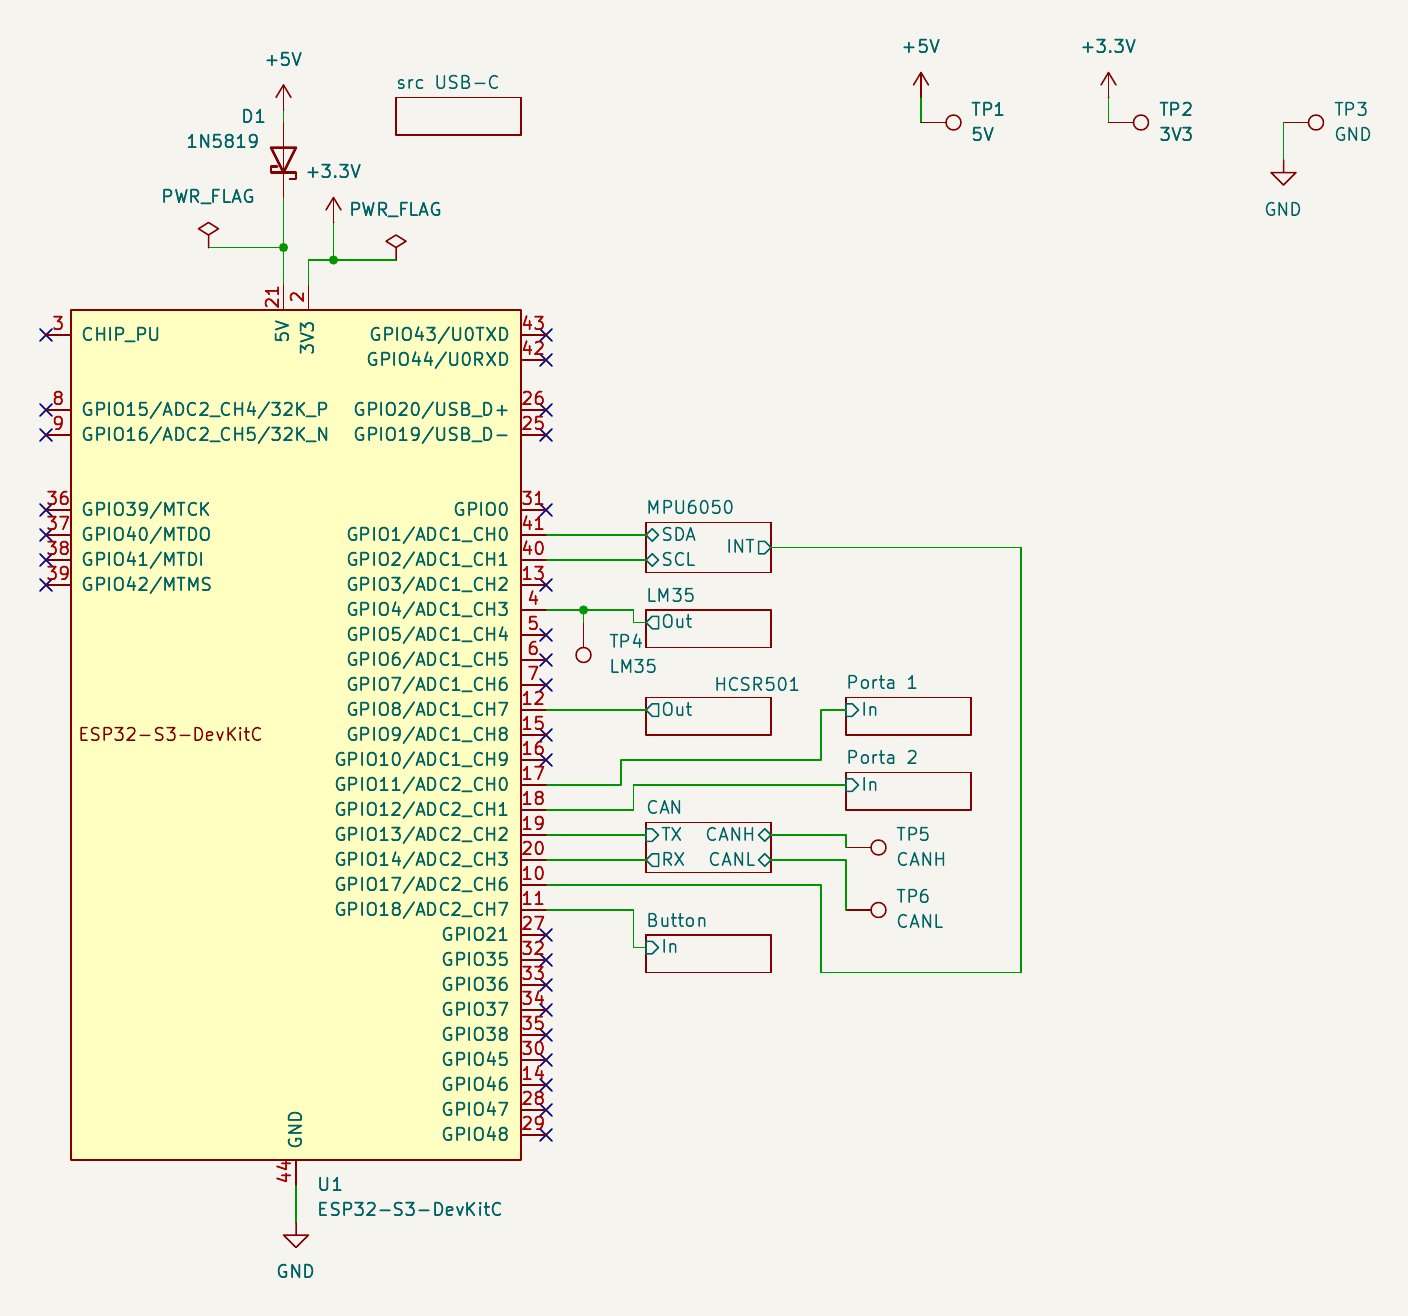
\includegraphics[width=0.9\linewidth]{figuras/esquema_p1.png}
\caption{Folha principal do esquemático: a DevKit (U1) e os blocos ligados aos seus pinos.}
\label{fig:esquema_raiz}
\end{figure}

\subsection{Layout}\label{sec:layout}

A placa mede \pcbLargura{} $\times$ \pcbAltura\,mm e tem duas camadas: as trilhas na face de
cima (F.Cu) e um plano de GND quase inteiro na de baixo (B.Cu), com alívio térmico nos
furos (Figuras~\ref{fig:pcb_3d} e~\ref{fig:pcb_camadas}). Os componentes são todos de furo
passante, para montagem à mão, e os módulos (DevKit, PIR, MPU, transceptor CAN, USB-C) entram
em barras de pinos fêmea. As decisões de posicionamento vieram da aula de projeto de PCB:

\begin{itemize}
  \item \textbf{Bloco analógico separado.} O LM35, o LM358 e o filtro RC ficam juntos, do
        lado do GPIO 4, longe do transceptor CAN e do I²C. A trilha do LM35 até o LM358 é
        curta, porque é o sinal pequeno (10\,mV/°C), e o RC fica colado no pino do ADC.
  \item \textbf{LM35 longe do calor.} Ele fica numa ponta da placa, longe da DevKit e do
        regulador, que esquentam com o Wi-Fi.
  \item \textbf{Antena livre.} Não há cobre embaixo da antena da DevKit, nas duas faces: o
        retângulo vazio no plano de GND da Figura~\ref{fig:pcb_camadas}.
  \item \textbf{PIR longe da antena}, na metade oposta da placa, por causa dos disparos falsos
        do HC-SR501 perto do Wi-Fi. O módulo fica deitado sobre a placa, com o domo para fora.
  \item \textbf{Plano de terra contínuo}, com o mínimo de fendas sob as trilhas de sinal, e
        100\,nF em cada pino de alimentação de CI.
\end{itemize}

\begin{figure}[H]
\centering
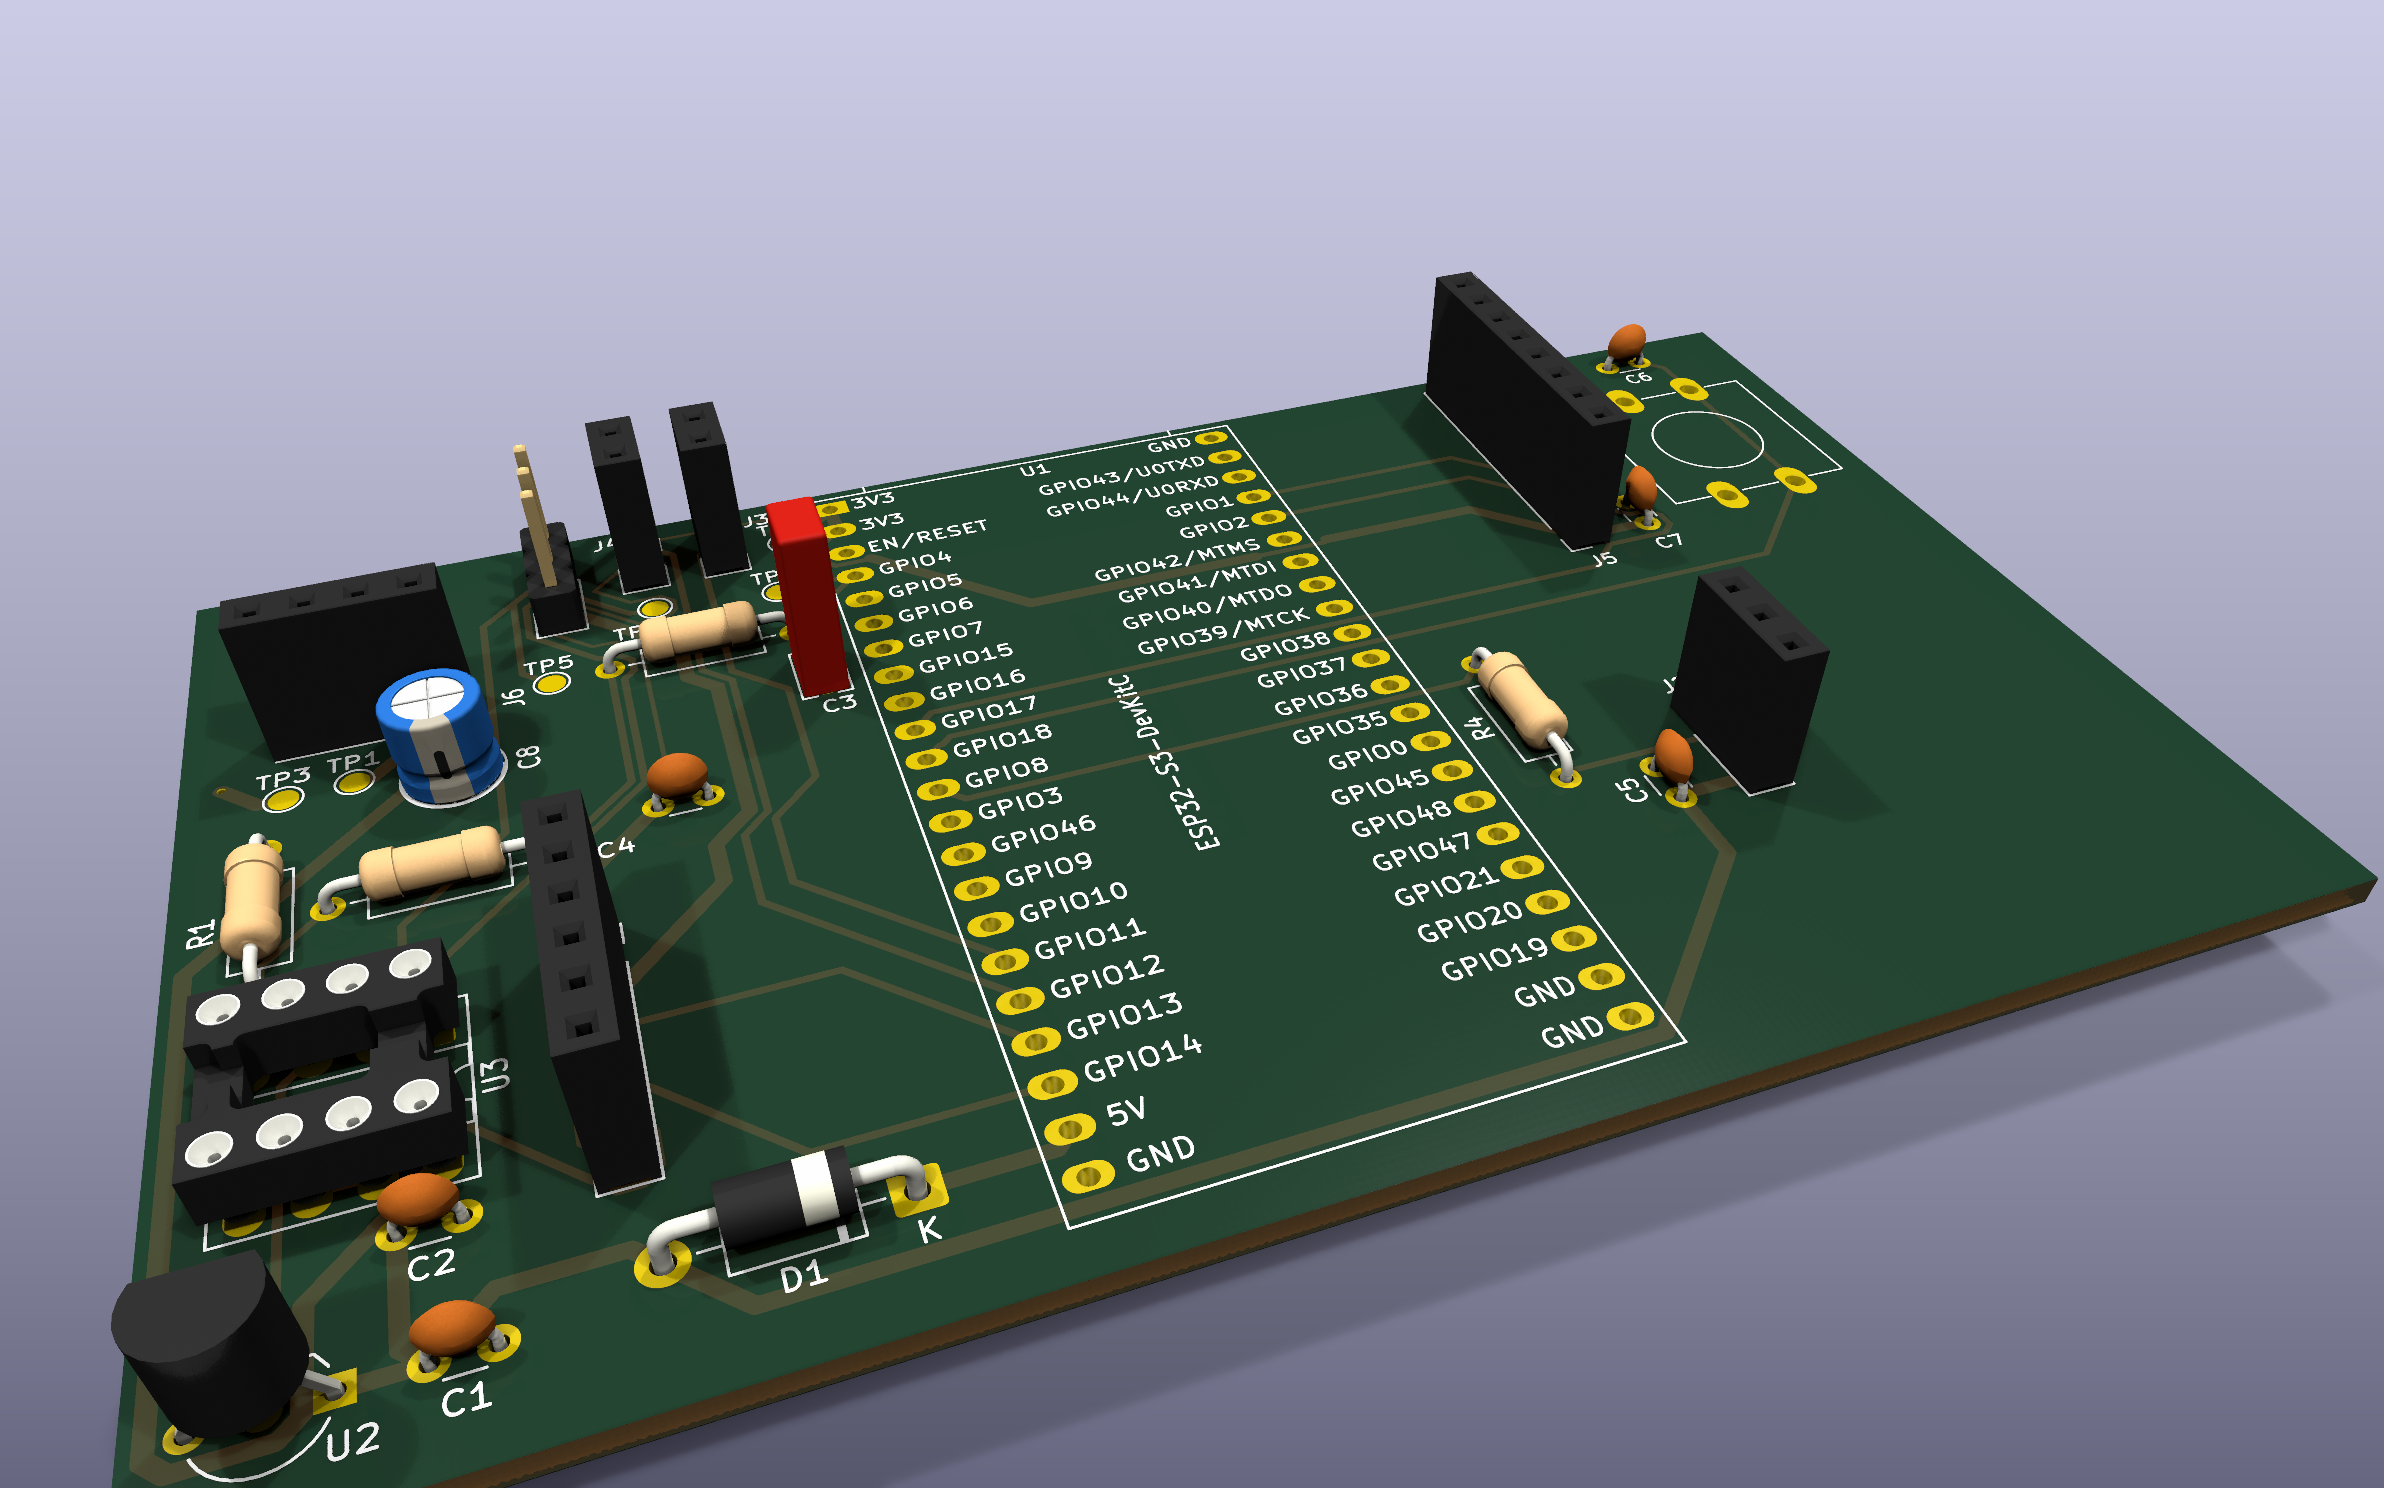
\includegraphics[width=0.9\linewidth]{figuras/pcb_3d_perspectiva.png}
\caption{Visualização 3D da PCB v1 (KiCad). O LM35 e o LM358 estão no canto de baixo à
esquerda; a DevKit, ao centro; o MPU-6050 e o botão, à direita.}
\label{fig:pcb_3d}
\end{figure}

\begin{figure}[H]
\centering
\begin{subfigure}[b]{0.49\linewidth}
  \centering
  \camada{\pcbTrimF}{\linewidth}{figuras/pcb_fcu.pdf}
  \caption{Face de cima: trilhas (F.Cu) e serigrafia.}
\end{subfigure}\hfill
\begin{subfigure}[b]{0.49\linewidth}
  \centering
  \camada{\pcbTrimB}{\linewidth}{figuras/pcb_bcu.pdf}
  \caption{Face de baixo (B.Cu), vista por baixo: plano de GND.}
\end{subfigure}
\caption{Camadas de cobre da PCB v1, exportadas do KiCad.}
\label{fig:pcb_camadas}
\end{figure}

\paragraph{Regras de projeto.} As regras ficam com folga sobre os limites da JLCPCB para
duas camadas (0,127\,mm de trilha e afastamento), pensando numa placa soldada à mão
(Tabela~\ref{tab:regras_pcb}).

\begin{table}[H]
\centering
\caption{Regras de projeto da PCB v1.}
\label{tab:regras_pcb}
\small
\begin{tabular}{@{}>{\raggedright\arraybackslash}p{6.2cm}>{\raggedright\arraybackslash}p{7.6cm}@{}}
\toprule
Item & Valor \\
\midrule
Afastamento e trilha mínimos & 0,2\,mm e 0,2\,mm \\
Trilhas de sinal & 0,4\,mm (0,25\,mm só em trecho apertado), afastamento de 0,25\,mm \\
Trilhas de alimentação (5\,V, 3,3\,V, GND) & 0,8\,mm; o pico de corrente é de $\sim$0,5\,A \\
Via & 0,8\,mm de diâmetro com furo de 0,4\,mm \\
Cobre até a borda & 0,5\,mm \\
Pads da DevKit & furo de 1,0\,mm, pad oval de 1,4 $\times$ 2,2\,mm: a barra de pinos tem 0,9\,mm de diagonal e não entrava no furo de 0,8\,mm do footprint original \\
Pads do LM35 & TO-92 de pads largos (1,5\,mm), para soldar à mão \\
Empilhamento & FR-4 de 1,6\,mm, cobre de 1\,oz (35\,µm) \\
\bottomrule
\end{tabular}
\end{table}

\subsection{Verificação e fabricação}

Antes de gerar os arquivos de fabricação, a placa passou por:
\begin{itemize}
  \item \textbf{ERC} (regras elétricas do esquemático): \ercViolacoes{} violações.
  \item \textbf{DRC} (regras de projeto do layout), com paridade com o esquemático:
        \drcErros{} erros, \drcSemLigacao{} ligações faltando e \drcParidade{} divergências
        com o esquema. Os \drcAvisos{} avisos são de serigrafia: o desenho da antena da DevKit
        passa da borda da placa, como esperado. Esses números são de uma rodada do
        \code{kicad-cli} feita para este relatório.
  \item \textbf{Teste no papel}: a placa impressa em escala 1:1, com as peças de verdade
        encaixadas por cima, para conferir o encaixe e a ordem dos pinos.
\end{itemize}

Os Gerbers e a furação foram gerados pelo \code{kicad-cli}, e a placa foi fabricada na
JLCPCB: duas camadas, FR-4 de 1,6\,mm, cobre de 1\,oz, 114 furos metalizados (nenhum sem
metalização) e acabamento HASL. A montagem é feita à mão. A lista de materiais tem \bomItens{} itens e
\bomPecas{} peças (Apêndice~\ref{ap:bom}).

\begin{figure}[H]
\centering
\begin{subfigure}[b]{0.49\linewidth}
  \centering
  \fotoouespaco{pcb_fabricada_cima}{\linewidth}{PCB v1 fabricada, face de cima}
\end{subfigure}\hfill
\begin{subfigure}[b]{0.49\linewidth}
  \centering
  \fotoouespaco{pcb_fabricada_baixo}{\linewidth}{PCB v1 fabricada, face de baixo}
\end{subfigure}
\caption{A PCB v1 como chegou da JLCPCB.}
\label{fig:pcb_fabricada}
\end{figure}

\subsection{Da PCB do primeiro semestre à v1}\label{sec:pcb_s1}

A primeira PCB do projeto, no fim do primeiro semestre, era de face simples, desenhada no
NI Ultiboard, e já juntava todos os sensores numa placa (Figura~\ref{fig:pcb_s1}). Ela serviu
para validar a integração, mas o mapa de pinos tinha quatro conflitos que só apareceram
depois: o LM35 no ADC2 (que não funciona com o Wi-Fi ligado), o CAN nos pinos do console
(UART0), uma porta no pino do LED da DevKit e o MPU-6050 em pinos da PSRAM. As regras da
Tabela~\ref{tab:regras_pinos} e a verificação na compilação existem por causa deles. A v1
também passou para duas camadas, com plano de terra, e trocou o amplificador simétrico por
alimentação simples.

\begin{figure}[H]
\centering
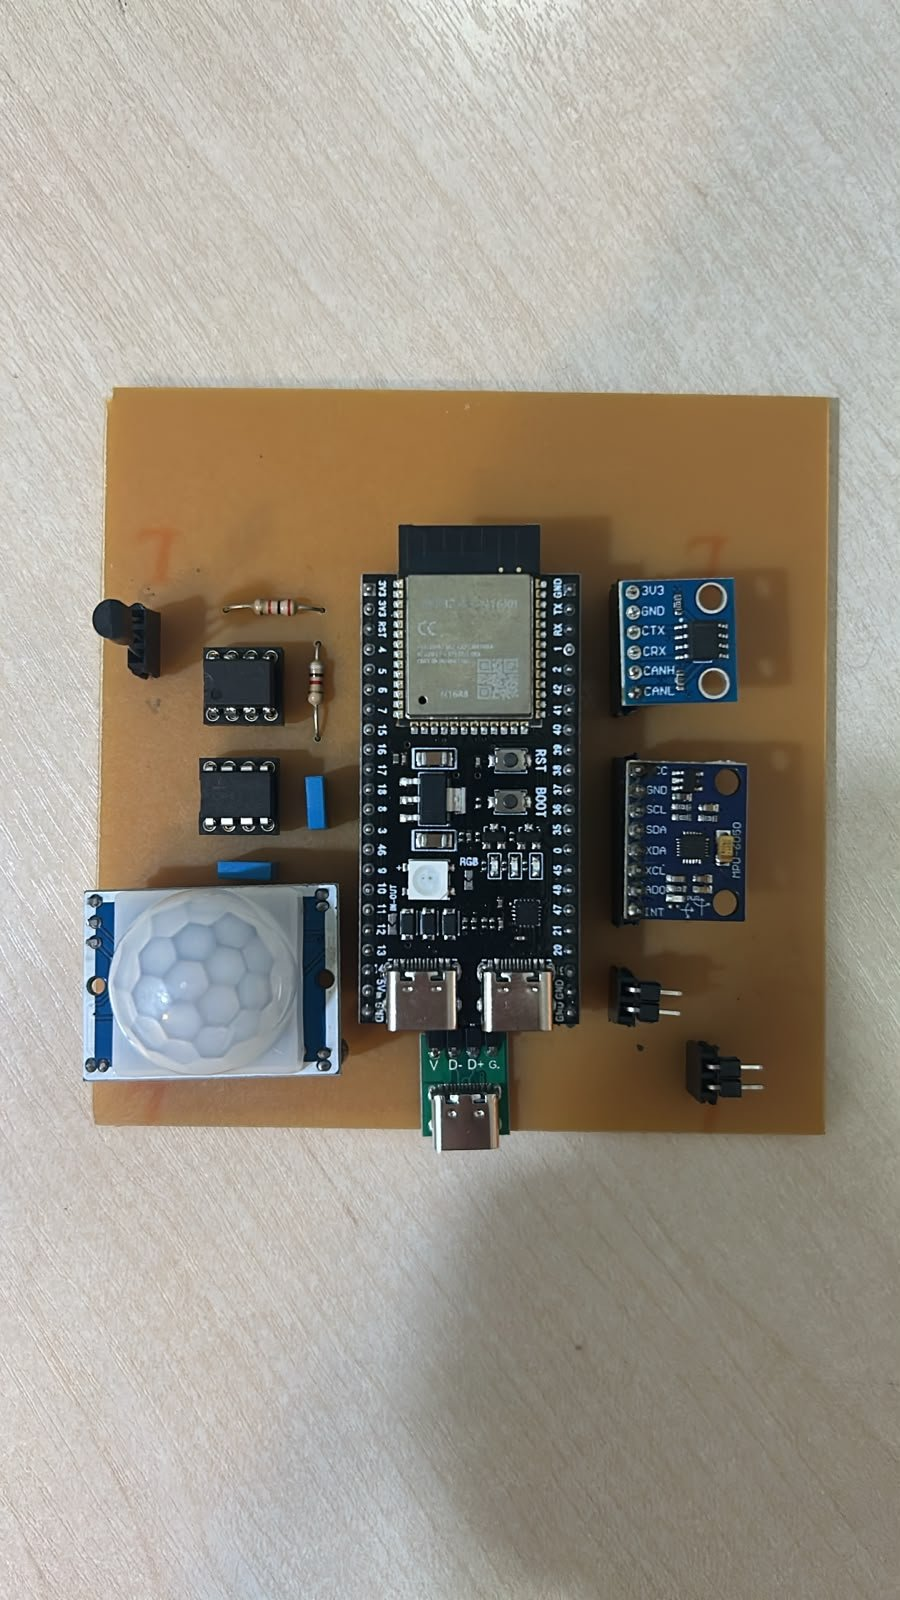
\includegraphics[height=7.5cm]{imagens/s1_pcb_montada.jpg}
\caption{A PCB de face simples do primeiro semestre, montada.}
\label{fig:pcb_s1}
\end{figure}
